\documentclass[aspectratio=169,10pt]{beamer}
\usetheme{Madrid}
\usepackage[T1]{fontenc}

\usepackage{fancybox,graphicx,hyperref,url}
\usepackage{tikz}
\usetikzlibrary{shapes,arrows}
\usetikzlibrary{positioning}
\usepackage{booktabs}
\usepackage{enumitem}

\usepackage{listings}
\usepackage{lstautogobble}
% Stolen from https://raw.githubusercontent.com/lammich/isabelle_llvm/2022/papers/ITP2022/lstisabelle.tex
% Not really meant for highlighting isabelle source, but for easily writing latex that looks like
% isabelle
%
% keyword level 1 - isabelle outer syntax
% keyword level 2 - isabelle inner syntax programming constructs (if, let, etc)
% keyword level 3 - standard constants (length, mod, etc)
% keyword level 4 - isabelle proof methods


% \newcommand{\lsem}{\ensuremath{\mathopen{[\![}}}
% \newcommand{\rsem}{\ensuremath{\mathclose{]\!]}}}

\lstdefinelanguage{isabelle}{
  morekeywords={theorem,theorems,corollary,lemma,lemmas,locale,sublocale,global_interpretation,begin,end,fixes,assumes,shows,and,class,
    constrains , definition, abbreviation, defines, where, done,unfolding, primrec, primcorec, inductive, coinductive, corecursive, corec, friend_of_corec, partial_function, fun, function, using, by, for, uses, file,
    schematic_lemma, concrete_definition, prepare_code_thms, export_code, datatype, codatatype, type_synonym, typedef, value,
    proof, next, qed, show, have, hence, thus, interpretation, fix, context, sepref_definition,is,export_llvm
 } ,
  morekeywords=[2]{rec, return, bind, foreach, if, then, else, do, let, in, res, spec, fail, assert, assume, while, case, of,
    check,with_split,npar,nseq},
  morekeywords=[3]{LNil, LCons, ltl, lhd, lnull, lmap, lset, Cons, None, Some, the, lfind, Logic, fold, produce, produce_inner, count_op, while_option, LEAST, ^^, snd, fst, produce_inner_aux, hd, tl,
    produce_1', produce_1, produce_induct, @, fproduce, comp_op, produce_comp_op_correctness, produce_1_comp_op_None_fproduce, skip_op, cong,
    ldropn, produce_1_comp_op_None_fproduce, WM, wmk, tmp, data, DT, insert, monotone, LConsR, LConsL, productive, EnvWM, EnvDT, LFinite, monotone_cong, monotone_cong_prepend, vimage, Suc,
    length, llength, set_t, tmps, drop, nth, coinduction, lfinite, llist_of, batch_op, filter, lfilter, incr_op, remdups, rev, map, List, map_filter, mset, case_event, Map, empty, lfilter, case_event, list_of,
    data_at, data_at_from_list, lcoll, coll, mono_prod, set, batch_coll_sound, get_Data, enat, ts, ws, batch_ts, lnth, batch_ts_sound, undefined, LNil_lprefix, LCons_lprefix, In_llist, Next_llist, in_llist,
    EZero, ESucc, ltake, pf_prod, pf_stop, pf_step, concat, snd, ltake_DT, the_enat, acc_batches, incr_batch_op, maxchain, paths, lpaths, incr_lcoll, incr_coll, sum, map_op, incr_hist_op,
    join_op, flatten_op, join_list, union_op, Inl, Inr, apply, Inl_leq, Inr_leq, incr_hist_op', eq_op, eq_op_lifted, WM, rel_prod, EQ, less_eq_sum, Pow, prefix, exit,
    monotone_cong_base, productive_cong, productive_cong_base, productive_cong_prepend, wms, lapp, lconcat, lprefix, lfilter, lshift, @@, lSup, THE},
%   morekeywords=[4]{simp,auto,intro,elim,rprems,refine_mono,refine_rcg},
  sensitive=True,
  morecomment=[s]{(\*}{\*)},
  moredelim=*[is][\ttfamily]{**}{**},
}


\DeclareTextCommand{\shortunderscore}{T1}{%
  \leavevmode \kern.06em\vbox{\hrule width.4em}}

\renewcommand{\textunderscore}{\shortunderscore}

\lstset{
    language=isabelle,
    upquote=true,
    mathescape=true,
    escapeinside={--"}{"},
    basicstyle={\itshape},
    keywordstyle=\rm\bfseries,
    keywordstyle=[2]\rm\tt,
    keywordstyle=[3]\rm\sffamily,
    keywordstyle=[4]\rm,
    keywordstyle=[5]\rm\bfseries,
    showstringspaces=false,
    keepspaces=true,
    columns=[c]fullflexible}
\lstset{literate=
  {"}{}0
%  {'}{{${}^\prime\!$}}1
  %{''}{{${}^\prime$}}1
  {'}{{${}^\prime$}}1
  {~:}{{$\notin$}}1
  {\%}{{$\lambda$}}1
  {\\\%}{{$\lambda$}}1
  {\\\$}{{$\mathbin{\,\$\,}$}}1
  {&}{{$\wedge$}}1
  {?}{{$\exists$}}1
%  {!}{{$\forall$}}1 clashes with nth xs!i
  {->}{{$\rightarrow$}}1
  {<-}{{$\leftarrow$}}1
%   {<.}{{$\langle$}}1
%   {.>}{{$\rangle$}}1
  {<=}{{$\le$}}1
  {>=}{{$\ge$}}1
  {<->}{{$\leftrightarrow$}}1
  {-->}{{$\longrightarrow$}}2
  {-->>}{{$\boldsymbol{\longrightarrow}$}}5
  {<-->}{{$\longleftrightarrow$}}1
  {=>}{{$\Rightarrow$}}1
  {==}{{$\equiv$}}2
  {==>}{{$\implies$}}2
  {<=>}{{$\Leftrightarrow$}}1
  {~=}{{$\ne$}}1
  {|}{{$\mid$}}1
  % {-`}{$vimage$}1
  {|`}{{$\restriction$}}1
  {!!}{{$\bigwedge$}}1
  {(}{{$($}}1
  {)}{{$)$}}1
  {\{}{{$\{$}}1
  {\}}{{$\}$}}1
  {[}{{$[$}}1
  {]}{{$]$}}1
  {[|}{{$\llbracket$}}1
  {|]}{{$\rrbracket$}}1
  {\\<lbrakk>}{{$\lsem$}}1
  {\\<rbrakk>}{{$\rsem$}}1
  {|-}{{$\vdash$}}1
  {|=}{{$\models$}}1
  {|->}{{$\mapsto$}}1
  {|_|}{{$\bigsqcup$}}1
  {...}{{$\dots$}}1
  {\\x}{{$\times$}}1
  {_0}{{${}_0$}}1
  {_1}{{${}_1$}}1
  {_2}{{${}_2$}}1
  {_3}{{${}_3$}}1
  {_4}{{${}_4$}}1
  {_5}{{${}_5$}}1
  {_6}{{${}_6$}}1
  {_7}{{${}_7$}}1
  {_8}{{${}_8$}}1
  {_9}{{${}_9$}}1
  {_L}{{${}_L$}}1
  {\\_n}{{${}_n$}}1
  {\\_i}{{${}_i$}}1
  {\\_j}{{${}_j$}}1
  {\\_x}{{${}_x$}}1
  {\\_y}{{${}_y$}}1
  {\\impl}{{${}_\dagger$}}1
  {^*}{{$^*$}}1
  {^k}{{$^k$}}1
  {^d}{{$^d$}}1
  {\\<^sup>*}{{$^*$}}1
  {\\<^sub>*}{{$_*$}}1
  {\\<^sub>A}{{$_A$}}1
  {\\<^sub>r}{{$_r$}}1
  {\\<^sub>a}{{$_a$}}1
  {:_i}{{$:_i$}}1
  {\\<A>}{{$\mathcal{A}$}}1
  {\\<O>}{{\sf o}}1
  {\\<Phi>}{{$\Phi$}}1
  {\\<phi>}{{$\phi$}}1
  {\\<Psi>}{{$\Psi$}}1
  {\\<sigma>}{{$\sigma$}}1
  {\\<Sigma>}{{$\Sigma$}}1
  {\\<cdot>}{{$\cdot$}}1
  {\\<in>}{{$\in$}}1
  {\\<le>}{{$\le$}}1
  {\\<noteq>}{{$\ne$}}1
  {\\<lambda>}{{$\lambda$}}1
  {\\<longrightarrow>}{{$\longrightarrow$}}1
  {\\<longleftrightarrow>}{{$\longleftrightarrow$}}1
  {\\<Rightarrow>}{{$\Rightarrow$}}1
  {\\<Longrightarrow>}{{$\Longrightarrow$}}1
  {\\<rightarrow>}{{$\rightarrow$}}1
  {\\<leftarrow>}{{$\leftarrow$}}1
  {\\<mapsto>}{{$\mapsto$}}1
  {\\<equiv>}{{$\equiv$}}1
  {\\<and>}{{$\wedge$}}1
  {\\<or>}{{$\vee$}}1
  {\\<And>}{{$\bigwedge$}}1
  {\\<Up>}{{$\Uparrow$}}1
  {\\<Down>}{{$\Downarrow$}}1
  {\\<Union>}{{$\bigcup$}}1
  {\\<up>}{{$\uparrow$}}1
  {\\<down>}{{$\downarrow$}}1
  {\\<times>}{{$\times$}}1
  {\\<forall>}{{$\forall$}}1
  {\\<exists>}{{$\exists$}}1
  {\\<nexists>}{{$\nexists$}}1
  {\\<union>}{{$\cup$}}1
  {\\<inter>}{{$\cap$}}1
  {\\in}{$\in$}1
  {\\union}{{$\cup$}}1
  {\\inter}{{$\cap$}}1
  {\\<subset>}{{$\subset$}}1
  {\\<subseteq>}{{$\subseteq$}}1
  {\\<supset>}{{$\supset$}}1
  {\\<supseteq>}{{$\supseteq$}}1
  {\\<alpha>}{{$\alpha$}}1
  {\\<beta>}{{$\beta$}}1
  {\\<gamma>}{{$\gamma$}}1
  {\\alpha}{{$\alpha$}}1
  {\\beta}{{$\beta$}}1
  {\\gamma}{{$\gamma$}}1
  {\\rho}{{$\rho$}}1
  {\\<rho>}{{$\rho$}}1
  {\\<Gamma>}{{$\Gamma$}}1
  {\\<langle>}{{$\langle$}}1
  {\\<rangle>}{{$\rangle$}}1
  {\\<not>}{{$\neg$}}1
  {\\<box>}{{$\oblong$}}1
  {\\<bot>}{{$\bot$}}1
  {\\<top>}{{$\top$}}1
  {\\<notin>}{{$\notin$}}1
  {\\<guillemotright>}{{$\gg$}}1
  {\\approx}{$\approx$}1
  {\\<approx>}{$\approx$}1
  {\\and}{$\wedge$}1
  {\\or}{$\vee$}1
  {\\mu}{$\mu$}1
  {\\Phi}{{$\Phi$}}1
  {\\Psi}{{$\Psi$}}1
  {\\le}{{$\le$}}1
  {\\Up}{{$\Uparrow$}}1
  {\\Down}{{$\Down$}}1
  {>>}{{$\gg$}}1
  {>>=}{{${\gg}{=}$}}1
  {<*lex*>}{{$\times_{\sf lex}$}}1
  {\\<open>}{{\rm\guilsinglleft}}1
  {\\<close>}{{\rm\guilsinglright}}1
  {\\<box>}{{$\square$}}1
  {\\<proof>}{{\color{darkgray}$\langle\text{proof}\rangle$}}7
}

\newcommand*{\rightcomment}[1]{\hfill\color{darkgray} --- #1}%

% \newcommand{\is}{\lstinline[language=isabelle,basicstyle=\normalsize\ttfamily\slshape]}
\newcommand{\is}{\lstinline[language=isabelle]}%, breaklines=true]}
\newcommand{\cs}{\lstinline[language=C++]}
\newcommand{\q}[1]{\mbox{\guilsinglleft{#1}\hspace{-.0pt}\guilsinglright}}
% \newcommand{\isai}[1]{\q{\lstinline[language=isabelle,basicstyle=\normalsize\ttfamily\slshape]{#1}}}
% \cMakeRobust

\usepackage[listings,skins,breakable,xparse]{tcolorbox}
\tcbuselibrary{theorems}
\tcbset{highlight math/.append style={boxrule=0pt,
                                      frame hidden,
                                      colback=yellow!40!white,
                                      sharp corners}}

\usepackage{xpatch}
\usepackage{xcolor}
\usepackage{realboxes}
\usetikzlibrary{fit}
\usetikzlibrary{shadings}
\usetikzlibrary{shapes.arrows,shadows.blur}

\pgfdeclarefunctionalshading{Hermite-Gaussian modes}{\pgfpoint{-25bp}{-25bp}}{\pgfpoint{25bp}{25bp}}{}{
    10 atan sin 1000 mul cos 1 add
    exch
    10 atan sin 1000 mul cos 1 add
    mul 4 div
    dup dup
}

\makeatletter
\xpretocmd\lstinline{\Colorbox{yellow!10!white}\bgroup\appto\lst@DeInit{\egroup}}{}{}
\makeatother

\definecolor{my_red}{RGB}{128, 0, 0}

\lstset{captionpos=b}
\lstset{numberbychapter=false}
\lstset{autogobble}
% \lstset{breaklines=true}

\usepackage{tikz}
\usepackage{subcaption}
\usetikzlibrary{calc, chains, decorations.pathmorphing}
\usetikzlibrary{shapes,arrows,backgrounds}
\usetikzlibrary{positioning,fit,shapes.geometric,shapes}

\setbeamercovered{transparent}

\setlistdepth{9}
\setlist[itemize,1]{label=$\bullet$}
\setlist[itemize,2]{label=$\bullet$}
\setlist[itemize,3]{label=$\bullet$}
\setlist[itemize,4]{label=$\bullet$}
\setlist[itemize,5]{label=$\bullet$}
\setlist[itemize,6]{label=$\bullet$}
\setlist[itemize,7]{label=$\bullet$}
\setlist[itemize,8]{label=$\bullet$}
\setlist[itemize,9]{label=$\bullet$}
\renewlist{itemize}{itemize}{9}

\setlist[enumerate,1]{label=$\arabic*.$}
\setlist[enumerate,2]{label=$\alph*.$}
\setlist[enumerate,3]{label=$\roman*.$}
\setlist[enumerate,4]{label=$\arabic*.$}
\setlist[enumerate,5]{label=$\alpha*$}
\setlist[enumerate,6]{label=$\roman*.$}
\setlist[enumerate,7]{label=$\arabic*.$}
\setlist[enumerate,8]{label=$\alph*.$}
\setlist[enumerate,9]{label=$\roman*.$}
\renewlist{enumerate}{enumerate}{9}

\AtBeginSection[]{
  \begin{frame}[noframenumbering]
    \vfill
    \centering
    \begin{beamercolorbox}[sep=8pt,center,shadow=true,rounded=true]{title}
      \usebeamerfont{title}\insertsectionhead\par%
    \end{beamercolorbox}
    \vfill
  \end{frame}
}

\title[Verified Time-Aware Stream Processing]{Verified Time-Aware Stream Processing}

\author[Rafael Castro]{
  Rafael Castro G. Silva\\\medskip
  {\small \url{rasi@di.ku.dk}}}

\date{02/11/2023}

\institute[UCPH]{
  Department of Computer Science \\
  University of Copenhagen}

\begin{document}

\begin{frame}
  \titlepage

\end{frame}

\begin{frame}[fragile]
  \frametitle{What is this PhD/Status seminar about?}
  \begin{itemize}
          \pause
    \item Distributed Systems
          \begin{itemize}
            \item Stream processing frameworks
                  \begin{itemize}
                    \item Dataflow models
                          \begin{itemize}
                            \item Time-Aware Computations
                          \end{itemize}
                  \end{itemize}
          \end{itemize}
          \pause
    \item Formal Methods
          \begin{itemize}
            \item Verification using proof assistants
                  \begin{itemize}
                    \item Isabelle proofs
                          \begin{itemize}
                            \item Verified + executable + efficient code
                          \end{itemize}
                  \end{itemize}
          \end{itemize}
    \item Formalization of Time-Aware Stream Processing
  \end{itemize}
\end{frame}

\begin{frame}{Contents}
  \begin{itemize}
    \item Introduction
    \item Preliminaries
    \item Lazy Lists Processors
    \item Time-Aware Operators
    \item Case Study
    \item Next Steps
  \end{itemize}
\end{frame}

\section{Introduction}

% TODO add references
% TODO check Dmitriys page
% https://www21.in.tum.de/~traytel/
% TODO finish this
\begin{frame}[fragile]
  \frametitle{Stream Processing}
  \begin{itemize}
    \item Stream Processing: Abstraction for processing data when the input is not completely presented in the begging of the computation
          \pause
    \item Dataflow Model:
          \begin{itemize}
            \item Directed graph of interconnected operators that perform event-wise transformations
            \item Examples: Apache Flink, Apache Samza, Apache Spark, Google Cloud Dataflow, and Timely Dataflow
                  \vspace*{-1ex}
                  \begin{figure}
                    \centering
                    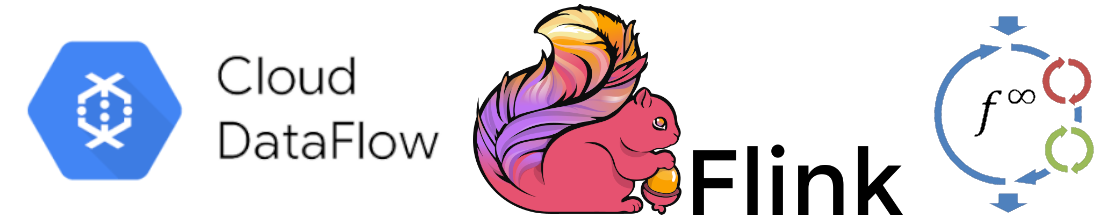
\includegraphics[scale=0.15]{all.png}
                  \end{figure}
                  \vspace*{-1ex}
            \item Highly Parallel
                  \vspace*{-1ex}
                  \begin{figure}
                    \begin{subfigure}{0.45\linewidth}
                      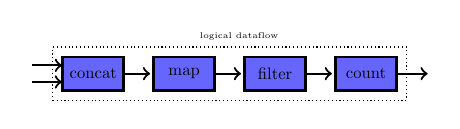
\begin{tikzpicture}[node distance = 0.6cm, scale=0.6, transform shape]]
                        \tikzstyle{operator} = [rectangle, draw, fill=blue!60, text width=3.0em, text centered, minimum height=20pt, line width=1pt]

                        \node [operator] at (0,0)  (concat) {concat};
                        \node [operator, right = of concat] (map) {map};
                        \node [operator, right = of map] (filter) {filter};
                        \node [operator, right = of filter] (count) {count};

                        \draw[<-,thick,shorten >=1pt] ([yshift=5pt]concat.west)  -- node[above]{} ++(-2em,0em);
                        \draw[<-,thick,shorten >=1pt] ([yshift=-5pt]concat.west)  -- node[above]{} ++(-2em,0em);
                        \draw [thick,->,shorten >=1pt] (concat) -- (map);
                        \draw [thick,->,shorten >=1pt] (map) -- (filter);
                        \draw [thick,->,shorten >=1pt] (filter) -- (count);
                        \draw[->,thick,shorten >=1pt] (count.east)  -- node[above]{} ++(2em,0em);

                        \node[draw,densely dotted, label={[xshift=2mm]above:{\tiny logical dataflow}},fit=(concat) (map) (filter) (count)] {};

                      \end{tikzpicture}
                    \end{subfigure}
                    \begin{subfigure}{0.45\linewidth}
                      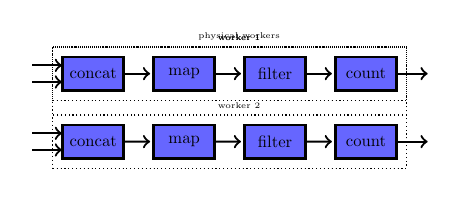
\begin{tikzpicture}[node distance = 0.6cm,auto, scale=0.6, transform shape]]
                        \tikzstyle{operator} = [rectangle, draw, fill=blue!60, text width=3.0em, text centered, minimum height=20pt, line width=1pt]

                        \node [operator] at (0,0)  (concat) {concat};
                        \node [operator, right = of concat] (map) {map};
                        \node [operator, right = of map] (filter) {filter};
                        \node [operator, right = of filter] (count) {count};

                        \draw[<-,thick,shorten >=1pt] ([yshift=5pt]concat.west)  -- node[above]{} ++(-2em,0em);
                        \draw[<-,thick,shorten >=1pt] ([yshift=-5pt]concat.west)  -- node[above]{} ++(-2em,0em);
                        \draw [thick,->,shorten >=1pt] (concat) -- (map);
                        \draw [thick,->,shorten >=1pt] (map) -- (filter);
                        \draw [thick,->,shorten >=1pt] (filter) -- (count);
                        \draw[->,thick,shorten >=1pt] (count.east)  -- node[above]{} ++(2em,0em);

                        \node[draw,densely dotted, label={[xshift=2mm]above:{\tiny worker 1}},fit=(concat) (map) (filter) (count)] {};

                        \node [operator, below=0.7cm of concat]  (concat') {concat};
                        \node [operator, right = of concat'] (map') {map};
                        \node [operator, right = of map'] (filter') {filter};
                        \node [operator, right = of filter'] (count') {count};

                        \draw[<-,thick,shorten >=1pt] ([yshift=5pt]concat'.west)  -- node[above]{} ++(-2em,0em);
                        \draw[<-,thick,shorten >=1pt] ([yshift=-5pt]concat'.west)  -- node[above]{} ++(-2em,0em);
                        \draw [thick,->,shorten >=1pt] (concat') -- (map');
                        \draw [thick,->,shorten >=1pt] (map') -- (filter');
                        \draw [thick,->,shorten >=1pt] (filter') -- (count');
                        \draw[->,thick,shorten >=1pt] (count'.east)  -- node[above]{} ++(2em,0em);

                        \node[draw,densely dotted, label={[xshift=2mm]above:{\tiny worker 1}},fit=(concat) (map) (filter) (count)] {};
                        \node[draw,densely dotted, label={[xshift=2mm]above:{\tiny worker 2}},fit=(concat') (map') (filter') (count')] {};
                        \node[draw,densely dotted, label={[xshift=2mm]above:{\tiny physical workers}},fit=(concat') (concat) (map') (filter') (count')] {};
                      \end{tikzpicture}
                    \end{subfigure}
                  \end{figure}
          \end{itemize}
                  \vspace*{-1ex}
    \item Time-Aware Computations
          \begin{itemize}
            \item Explain watermarks
          \end{itemize}
    \item Bugs in Stream Processing
  \end{itemize}
\end{frame}

\section{Preliminaries}
\begin{frame}[fragile]
  \frametitle{Isabelle/HOL}
  \begin{itemize}
    \item Classical higher-order logic (HOL): Simple Typed Lambda Calculus + (Hilbert) axiom of choice + axiom of infinity + rank-1 polymorphism
    \item Isabelle: A generic proof assistant
          \begin{figure}
            \centering
            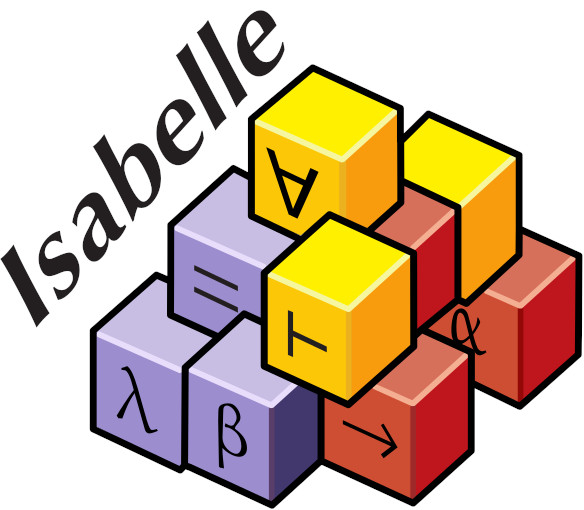
\includegraphics[scale=0.15]{isabelle}
          \end{figure}
    \item Isabelle/HOL: Isabelle's flavor of HOL
    \item All functions in Isabelle/HOL must be total
  \end{itemize}
\end{frame}

\begin{frame}[fragile]
  \frametitle{Isabelle/HOL: (Co)datatypes}
  \begin{itemize}
    \item Datatypes and Codatatypes
\vspace*{-1ex}
          \begin{tcblisting}{hbox,listing only,listing options={language=isabelle,aboveskip=0pt,belowskip=0pt},size=fbox,boxrule=0pt,frame hidden,arc=0pt,colback=yellow!10!white}
codatatype (lset: 'a) llist = lnull: LNil | LCons (lhd: 'a) (ltl: "'a llist")
  for map: lmap where "ltl LNil = LNil"
          \end{tcblisting}
\vspace*{-1ex}
    \item Examples:
\vspace*{-1ex}
          \begin{itemize}
            \item \is{LNil}
            \item \is{LCons 1 (LCons 2 (LCons 3 LNil))}
            \item \is{LCons 0 (LCons 0 (LCons 0 (...)))}
          \end{itemize}
\vspace*{-1ex}
          \pause
    \item Induction principle assuming membership in the lazy list
    \item Coinductive principle for lazy list equality:
          \begin{itemize}
            \item Show that there is a pair of goggles that makes them to look the same, which implies that:
                  \begin{itemize}
                    \item The first lazy list if empty iff second is
                    \item They have the same head
                    \item Their tail looks the same
                  \end{itemize}
          \end{itemize}
  \end{itemize}
\vspace*{-1ex}
  \begin{figure}
    \centering
    
\includegraphics[scale=0.4]{equality_1.png}
  \end{figure}
\end{frame}

\begin{frame}[fragile,noframenumbering]
  \frametitle{Isabelle/HOL: (Co)datatypes}
  \begin{itemize}
    \item Datatypes and Codatatypes
\vspace*{-1ex}
          \begin{tcblisting}{hbox,listing only,listing options={language=isabelle,aboveskip=0pt,belowskip=0pt},size=fbox,boxrule=0pt,frame hidden,arc=0pt,colback=yellow!10!white}
codatatype (lset: 'a) llist = lnull: LNil | LCons (lhd: 'a) (ltl: "'a llist")
  for map: lmap where "ltl LNil = LNil"
          \end{tcblisting}
\vspace*{-1ex}
    \item Examples:
\vspace*{-1ex}
          \begin{itemize}
            \item \is{LNil}
            \item \is{LCons 1 (LCons 2 (LCons 3 LNil))}
            \item \is{LCons 0 (LCons 0 (LCons 0 (...)))}
          \end{itemize}
\vspace*{-1ex}
    \item Induction principle assuming membership in the lazy list
    \item Coinductive principle for lazy list equality:
          \begin{itemize}
            \item Show that there is a pair of goggles that makes them to look the same, which must imply that:
                  \begin{itemize}
                    \item The first lazy list if empty iff second is
                    \item They have the same head
                    \item Their tail looks the same
                  \end{itemize}
          \end{itemize}
  \end{itemize}
\vspace*{-1ex}
  \begin{figure}
    \centering
    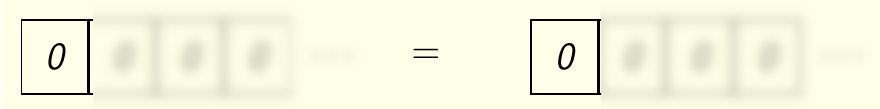
\includegraphics[scale=0.4]{equality_2.png}
  \end{figure}
\end{frame}

% TODO add notes for explaining codatatype command
\begin{frame}[fragile,noframenumbering]
  \frametitle{Isabelle/HOL: (Co)datatypes}
  \begin{itemize}
    \item Datatypes and Codatatypes
\vspace*{-1ex}
          \begin{tcblisting}{hbox,listing only,listing options={language=isabelle,aboveskip=0pt,belowskip=0pt},size=fbox,boxrule=0pt,frame hidden,arc=0pt,colback=yellow!10!white}
codatatype (lset: 'a) llist = lnull: LNil | LCons (lhd: 'a) (ltl: "'a llist")
  for map: lmap where "ltl LNil = LNil"
          \end{tcblisting}
\vspace*{-1ex}
    \item Examples:
\vspace*{-1ex}
          \begin{itemize}
            \item \is{LNil}
            \item \is{LCons 1 (LCons 2 (LCons 3 LNil))}
            \item \is{LCons 0 (LCons 0 (LCons 0 (...)))}
          \end{itemize}
    \item Induction principle assuming membership in the lazy list
    \item Coinductive principle for lazy list equality:
          \begin{itemize}
            \item Show that there is a pair of goggles that makes them to look the same, which must imply that:
                  \begin{itemize}
                    \item The first lazy list if empty iff second is
                    \item They have the same head
                    \item Their tail looks the same
                  \end{itemize}
          \end{itemize}
  \end{itemize}
\vspace*{-1ex}
  \begin{figure}
    \centering
    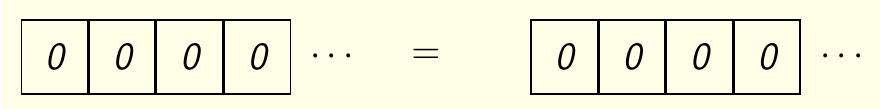
\includegraphics[scale=0.4]{equality.png}
  \end{figure}
\end{frame}

\begin{frame}[fragile]
  \frametitle{Isabelle/HOL: Recursion and While Combinator}
  \begin{itemize}
    \item Recursion

\begin{tcblisting}{hbox,listing only,listing options={language=isabelle,aboveskip=0pt,belowskip=0pt},size=fbox,boxrule=0pt,frame hidden,arc=0pt,colback=yellow!10!white}
fun lshift :: "'a list => 'a llist => 'a llist" (infixr @@ 65) where
  "lshift [] lxs = lxs"
| "lshift (x # xs) lxs = LCons x (lshift xs lxs)"
\end{tcblisting}
  \item While Combinator
\begin{tcblisting}{hbox,listing only,listing options={language=isabelle,aboveskip=0pt,belowskip=0pt},size=fbox,boxrule=0pt,frame hidden,arc=0pt,colback=yellow!10!white}
definition while_option :: "('a => bool) => ('a => 'a) => 'a => 'a option" where
"while_option b c s = $\ldots$"
\end{tcblisting}
    \item While rule for invariant reasoning (hoare-style):
          \begin{itemize}
            \item There is something that holds before a step; that thing still holds after the step
          \end{itemize}
          \end{itemize}
\end{frame}

\begin{frame}[fragile]
  \frametitle{Isabelle/HOL: Corecursion and Friends}
  \begin{itemize}
          \item Corecursion is like recursion, but instead of always eventually reducing an argument it always eventually produces something
          \pause
    \item Corec:
\vspace*{-1ex}
\begin{tcblisting}{hbox,listing only,listing options={language=isabelle,aboveskip=0pt,belowskip=0pt},size=fbox,boxrule=0pt,frame hidden,arc=0pt,colback=yellow!10!white}
corec lapp :: "'a llist => 'a llist => 'a llist" where
  "lapp lxs lys = case lxs of LNil => lys | LCons x lxs' => LCons x (lapp lxs' lys)"
\end{tcblisting}
\vspace*{-1ex}
          \pause
    \item Friendly function
          \begin{itemize}
            \item Preserves productivity: it may consume at most one constructor to produce one constructor.
          \end{itemize}
\vspace*{-1ex}
\begin{tcblisting}{hbox,listing only,listing options={language=isabelle,aboveskip=0pt,belowskip=0pt},size=fbox,boxrule=0pt,frame hidden,arc=0pt,colback=yellow!10!white}
friend_of_corec lshift where
  "xs @@ lxs = (case xs of
    [] => (case lxs of LNil => LNil | LCons x lxs' => LCons x lxs')
  | x#xs' => LCons x (xs' @@ lxs))"
  by (auto split: list.splits llist.splits) (transfer_prover)

lconcat lxs = case lxs of LNil => LNil | LCons xs lxs' => lshift xs (lconcat lxs')
\end{tcblisting}
\vspace*{-1ex}
          \pause
          \item Coinduction up to congruence: Coinduction for Lazy list equality can be extended to compare an entire finite prefix through a congruence relation
  \end{itemize}
\end{frame}

\begin{frame}[fragile]
  \frametitle{Isabelle/HOL: (Co)inductive Predicates}
  \begin{itemize}
    \item Inductive predicate
          \begin{itemize}
            \item Finite number of introduction rule applications
          \end{itemize}
\begin{tcblisting}{hbox,listing only,listing options={language=isabelle,aboveskip=0pt,belowskip=0pt},size=fbox,boxrule=0pt,frame hidden,arc=0pt,colback=yellow!10!white}
inductive in_llist :: "'a => 'a llist => bool" where
    In_llist: "in_llist x (LCons x lxs)"
  | Next_llist: "in_llist x lxs => in_llist x (LCons y lxs)"

in_llist 2 (LCons 1 (LCons (2 (...))))
\end{tcblisting}
          \pause
    \item Coinductive predicate
          \begin{itemize}
            \item Infinite number of introduction rule applications
          \end{itemize}
\begin{tcblisting}{hbox,listing only,listing options={language=isabelle,aboveskip=0pt,belowskip=0pt},size=fbox,boxrule=0pt,frame hidden,arc=0pt,colback=yellow!10!white}
coinductive lprefix :: "'a llist => 'a llist => bool" where
    LNil_lprefix: "lprefix LNil lys"
  | LCons_lprefix: "lprefix lxs lys => lprefix (LCons x lxs) (LCons x lys)"

lprefix (LCons 1 (LCons (2 (...)))) (LCons 1 (LCons (2 (...))))
\end{tcblisting}
          \pause
    \item Coinduction principle
    \item But not coinduction up to congruence for free
  \end{itemize}
\end{frame}

\section{Lazy Lists Processors}

\begin{frame}[fragile]
  \frametitle{Operator formalization}
  \begin{itemize}
    \item Operator as a codatatype
          \begin{itemize}
            \item Taking \is{'i} as the input type, and \is{'o} as the output type:
\vspace*{-1.5ex}
\begin{tcblisting}{hbox,listing only,listing options={language=isabelle,aboveskip=0pt,belowskip=0pt},size=fbox,boxrule=0pt,frame hidden,arc=0pt,colback=yellow!10!white}
codatatype ('o, 'i) op = Logic ("apply": "('i => ('o, 'i) op $\times$ 'o list)")
\end{tcblisting}
\vspace*{-1.5ex}
          \pause
            \item Infinite trees: applying the selector \is{apply} ``walks'' a branch of the tree
          \end{itemize}
  \end{itemize}
\end{frame}

% TODO add some figure showing the tree
\begin{frame}[fragile]
  \frametitle{Execution formalization}
  \begin{itemize}
    \item Produce function: applies the logic (co)recursively throughout a lazy list
\vspace*{-1.5ex}
\begin{tcblisting}{hbox,listing only,listing options={language=isabelle,aboveskip=0pt,belowskip=0pt},size=fbox,boxrule=0pt,frame hidden,arc=0pt,colback=yellow!10!white}
definition "produce_1' op lxs = while_option
  ($\lambda$(op, lxs). \<not> lnull lxs \<and> snd (apply op (lhd lxs)) = [])
  ($\lambda$(op, lxs). (fst (apply op (lhd lxs)), ltl lxs)) (op, lxs)"
definition "produce_1 op lxs =
  (case produce_1' op lxs of None => None
  | Some (op', lxs') => if lnull lxs' then None else
    let (op'', out) = apply op' (lhd lxs') in Some (op'', hd out, tl out, ltl lxs'))"
corec produce where
  "produce op lxs = (case produce_1 op lxs of None => LNil
    | Some (op', x, xs, lxs') => LCons x (xs @@ produce op' lxs'))"
\end{tcblisting}
\vspace*{-1.5ex}
          \pause
          \item \is{produce_1} has an induction principle based on the while invariant rule
  \end{itemize}
\end{frame}

\begin{frame}[fragile]
  \frametitle{Operators: Count}
  \begin{itemize}
    \item Example:
\begin{tcblisting}{hbox,listing only,listing options={language=isabelle,aboveskip=0pt,belowskip=0pt},size=fbox,boxrule=0pt,frame hidden,arc=0pt,colback=yellow!10!white}
corec count_op where "count_op P n =
  Logic ($\lambda$e. if P e then (count_op P (n + 1), [n+1]) else (count_op P n, []))"
\end{tcblisting}
  \end{itemize}
  \begin{figure}[!t]
    \centering
    \begin{tikzpicture}[scale=0.9, every node/.style={scale=0.9}]
      \begin{scope}[local bounding box=scope1]
        \node[] (0,0) (s1) {\text{\is{stream_2}}};
        \node[right = 0.0cm of s1] (eq) {$=$};
      \end{scope}
      \begin{scope}[shift={($(scope1.east)+(0.8cm,0)$)}]
        \tikzset{tape/.style={minimum size=.6cm, draw}}
        \begin{scope}[start chain=0 going right, node distance=0mm]
          \foreach \x [count=\i] in {\is{0},\is{3},\is{3},\is{6}, \is{24}} {
            \node [on chain=0, tape] (a\i) {\x};
          }
        \end{scope}
      \end{scope}

      \begin{scope}[shift={($(scope1.center)+(-2.2cm,-1cm)$)},local bounding box=scope3]
        \node[] (0,0) (prod) {\text{\is{produce (count_op is_even 0)}}};
        \node[right = 0.0cm of prod] (s1) {\text{\is{stream_2}}};
        \node[right = 0.0cm of s1] (eq) {$=$};
      \end{scope}
      \begin{scope}[shift={($(scope3.east)+(0.9cm,0)$)}]
        \tikzset{tape/.style={minimum size=.6cm, draw}}
        \begin{scope}[start chain=0 going right, node distance=0mm]
          \foreach \x [count=\i] in {\is{1},\is{2}, \is{3}} {
            \node [on chain=0, tape] (b\i) {\x};
          }
        \end{scope}
      \end{scope}
      \draw[->, thick]  (a1.south) -- (b1.north);
      \draw[->, thick]  (a4.south) -- (b2.north);
      \draw[->, thick]  (a5.south) -- (b3.north);
    \end{tikzpicture}
  \end{figure}
\end{frame}

\begin{frame}[fragile]
  \frametitle{Sequential Composition}
  \begin{itemize}
    \item Sequential composition: take the output of the first operator and give it as input to the second operator.
\vspace*{-1ex}
\begin{tcblisting}{hbox,listing only,listing options={language=isabelle,aboveskip=0pt,belowskip=0pt},size=fbox,boxrule=0pt,frame hidden,arc=0pt,colback=yellow!10!white}
definition "fproduce op xs = fold ($\lambda$e (op, out).
  let (op', out') = apply op e in (op', out @ out')) xs (op, [])"
corec comp_op where
  "comp_op op_1 op_2 = Logic ($\lambda$ev.
     let (op_1', out) = apply op_1 ev;  (op_2', out') = fproduce op_2 out
     in (comp_op op_1' op_2', out'))"
\end{tcblisting}
  \end{itemize}
\end{frame}

\begin{frame}[fragile]
  \frametitle{Sequential Composition: Correctness}
  \begin{itemize}
    \item Correctness:
\vspace*{-1ex}
\begin{tcblisting}{hbox,listing only,listing options={language=isabelle,aboveskip=0pt,belowskip=0pt},size=fbox,boxrule=0pt,frame hidden,arc=0pt,colback=yellow!10!white}
"produce (comp_op op_1 op_2) lxs = produce op_2 (produce op_1 lxs)"
\end{tcblisting}
\vspace*{-1ex}
          \pause
            \item Proof: coinduction principle for lazy list equality and \is{produce_1} induction principle
                  \begin{itemize}
          \pause
                    \item Generalization: we must be able to reason about elements in arbitrary positions
\vspace*{-1ex}
\begin{tcblisting}{hbox,listing only,listing options={language=isabelle,aboveskip=0pt,belowskip=0pt},size=fbox,boxrule=0pt,frame hidden,arc=0pt,colback=yellow!10!white}
corec skip_op where
  "skip_op op n = Logic ($\lambda$ev. let (op', out) = apply op ev in
     if length out < n then (skip_op op' (n - length out), [])
     else (op', drop n out))"
\end{tcblisting}
\vspace*{-1ex}
          \pause
                    \item Correctness: Coinduction up to congruence for lazy list equality
  \end{itemize}
  \end{itemize}
\end{frame}

\section{Time-Aware Operators}

\begin{frame}[fragile]
  \frametitle{Time-Aware Streams}
  \begin{itemize}
    \item Time-Aware lazy lists
\vspace*{-1ex}
\begin{tcblisting}{hbox,listing only,listing options={language=isabelle,aboveskip=0pt,belowskip=0pt},size=fbox,boxrule=0pt,frame hidden,arc=0pt,colback=yellow!10!white}
datatype ('t::order, 'd) event = DT (tmp: 't) (data: 'd) | WM (wmk: 't)
\end{tcblisting}
\vspace*{-1ex}
          \pause
    \item Generalization to partial orders
          \begin{itemize}
            \item Cycles
            \item Operators with multiple inputs
          \end{itemize}
    \end{itemize}
\end{frame}

\begin{frame}[fragile]
  \frametitle{Monotone Time-Aware Streams}
  \begin{itemize}
    \item Monotone: watermarks do not go back in time
\vspace*{-1ex}
\begin{tcblisting}{hbox,listing only,listing options={language=isabelle,aboveskip=0pt,belowskip=0pt},size=fbox,boxrule=0pt,frame hidden,arc=0pt,colback=yellow!10!white}
coinductive monotone :: "('t::order, 'd) event llist => 't set => bool" where
  LNil: "monotone LNil W"
| LConsR: "($\forall$wm' $\in$ W. \<not> wm' >= wm) --> monotone lxs ({wm} $\cup$ W) -->
   monotone (LCons (WM wm) lxs) W"
| LConsL: "($\forall$wm $\in$ W. \<not> wm >= t) --> monotone lxs W -->
   monotone (LCons (DT t d) lxs) W"
\end{tcblisting}
\vspace*{-1ex}
          \pause
          \item Up to congruence coinduction principle
          \pause
    \item Example:
  \end{itemize}

  \begin{figure}[!t]
    \begin{subfigure}{.5\textwidth}
      \raggedright
      \begin{tabular}{@{}l@{}}
        \text{\is{stream_3 =}}
        \\
        \begin{tikzpicture}[scale=0.9, every node/.style={scale=0.9},background rectangle/.style={fill=yellow!10!white},show background rectangle]
          \tikzset{tape/.style={minimum size=.6cm, draw}}
          \begin{scope}[start chain=0 going right, node distance=0mm]
            \foreach \x [count=\i] in {\is{DT t_4 **d**},\is{DT t_0 **a**},\is{DT t_1 **c**},\is{WM t_1},\is{DT t_5 **c**}} {
              \ifnum\i=5
                \node [on chain=0, tape, outer sep=0pt] (n\i) {\x};
                \draw (n\i.north east) -- ++(.1,0) decorate [decoration={zigzag, segment length=.12cm, amplitude=.02cm}] {-- ($(n\i.south east)+(+.1,0)$)} -- (n\i.south east) -- cycle;
              \else
                \node [on chain=0, tape] (n\i) {\x};
              \fi
            }
          \end{scope}
        \end{tikzpicture}
        \vspace*{-1.3ex}
        \\
        \begin{tikzpicture}[scale=0.9, every node/.style={scale=0.9},background rectangle/.style={fill=yellow!10!white},show background rectangle]
          \tikzset{tape/.style={minimum size=.6cm, draw}}
          \begin{scope}[start chain=0 going right, node distance=0mm]
            \foreach \x [count=\i] in {\is{DT t_3 **a**},\is{DT t_5 **a**},\is{WM t_2},\is{WM t_5},\is{DT t_2 **b**}} {
              \ifnum\i=5
                \node [on chain=0, tape, outer sep=0pt] (n\i) {\x};
                \draw (n\i.north east) -- ++(.1,0) decorate [decoration={zigzag, segment length=.12cm, amplitude=.02cm}] {-- ($(n\i.south east)+(+.1,0)$)} -- (n\i.south east) -- cycle;
              \else
                \node [on chain=0, tape] (n\i) {\x};
              \fi
              \ifnum\i=1
                \draw (n\i.north west) -- ++(-0.1,0) decorate [decoration={zigzag, segment length=0.12cm, amplitude=.02cm}] {-- ($(n\i.south west)+(-.1,0)$)} -- (n\i.south west) -- cycle;
              \fi
            }
            \node [right=.05cm of n5] {$\cdots$};
          \end{scope}
        \end{tikzpicture}
      \end{tabular}
      \label{fig:stream_example_1}
    \end{subfigure}
    \begin{subfigure}{.38\textwidth}
      \begin{tikzpicture}[style={grow'=up,level distance=3em, sibling distance=2em}, level distance=8mm,background rectangle/.style={fill=yellow!10!white},show background rectangle]
        \node (t0) at (-0.8,0) {$C_{t_{0}}$: \{\is{**a**}\}};
        \node (t1) at (-2.5,1) {$C_{t_{1}}$: \{\is{**c**}\}};
        \node (t2) at (-0.8,1) {$C_{t_{2}}$: \{\is{**b**}\}};
        \node (t3) at (0.8,1) {$C_{t_{3}}$: \{\is{**a**}\}};
        \node (t4) at (-2.5,2) {$C_{t_{4}}$: \{\is{**d**}\}};
        \node (t5) at (0.0,2) {$C_{t_{5}}$: \{\is{**a**,**c**}\}};

        \path [->] (t0) edge node {} (t1);
        \path [->] (t0) edge node {} (t2);
        \path [->] (t0) edge node {} (t3);
        \path [->] (t3) edge node {} (t5);
        \path [->] (t1) edge node {} (t4);
        \path [->] (t2) edge node {} (t5);
      \end{tikzpicture}
      \label{fig:diamond_order}
    \vspace*{-2ex}
  \end{subfigure}
  \end{figure}
\end{frame}


\begin{frame}[fragile]
  \frametitle{Productive Time-Aware Streams}
  \begin{itemize}
    \item Productive: always eventually allows the production
          \pause
          \begin{itemize}
            \item Batching operators: accumulate data until its completion
          \pause
            \item Data is always eventually completed by some watermark
\vspace*{-1ex}
\begin{tcblisting}{hbox,listing only,listing options={language=isabelle,aboveskip=0pt,belowskip=0pt},size=fbox,boxrule=0pt,frame hidden,arc=0pt,colback=yellow!10!white}
coinductive productive where
  LFinite: "lfinite lxs --> productive lxs"
| EnvWM: "\<not> lfinite lxs --> (?u $\in$ vimage WM (lset lxs). u >= t) -->
   productive lxs --> productive (LCons (DT t d) lxs)"
| SkipWM: "\<not> lfinite lxs --> productive lxs -->
   productive (LCons (WM t) lxs)"
\end{tcblisting}
\vspace*{-1ex}
          \pause
          \item Up to congruence coinduction principle
          \end{itemize}
  \end{itemize}
\end{frame}

\begin{frame}[fragile]
  \frametitle{Building Blocks: Batch Operator}

\end{frame}

\begin{frame}[fragile]
  \frametitle{Batch Operator: Soundness}

\end{frame}

\begin{frame}[fragile]
  \frametitle{Batch Operator: Completeness}
  \begin{itemize}
    \item Uses soundness of \is{batch_op}
    \item Proof by induction over n
  \end{itemize}

  \begin{tcolorbox}[ams align,colback=yellow!10!white,colframe=my_red]
    \hspace*{-0.6cm}
  \begin{array}{@{}l@{}}
    \text{\is{mono_prod lxs W --> (?i d. enat i < llength lxs \\<and> lnth lxs i = DT t d \\<and> n = Suc i) \\<or>}}
    \\
    \text{\is{n = 0 \\<and> t \\in set_t buf --> (\\<forall>t' \\in set_t buf. lfinite lxs \\<or> ?wm >= t' . WM wm \\in lset lxs) -->>}}
    \\
    \text{\is{?wm batch. DT wm batch \\in lset (produce (batch_op buf) lxs) \\<and> t \\in set_t batch \\<or>}}
    \\
    \text{\is{(\\<forall>k  \\in \{n ..< the_enat (llength lxs)\} . \\<not> (?t' >= t. lnth lxs k = WM t')) \\<and> lfinite lxs}}
  \end{array}
  \end{tcolorbox}
\end{frame}

\begin{frame}[fragile]
  \frametitle{Batch Operator: Monotone}

\end{frame}

\begin{frame}[fragile]
  \frametitle{Batch Operator: Productive}

\end{frame}

\begin{frame}[fragile]
  \frametitle{Building Blocks: Incremental Operator}

\end{frame}

\begin{frame}[fragile]
  \frametitle{Batch Operator: Soundness}

\end{frame}

\begin{frame}[fragile]
  \frametitle{Batch Operator: Completeness}

\end{frame}

\begin{frame}[fragile]
  \frametitle{Batch Operator: Monotone}

\end{frame}

\begin{frame}[fragile]
  \frametitle{Batch Operator: Productive}

\end{frame}

\begin{frame}[fragile]
  \frametitle{Compositional Reasoning}

\end{frame}

\section{Case Study}

\begin{frame}
  \frametitle{Histogram}
\end{frame}

\begin{frame}
  \frametitle{Histogram: Soundness}

\end{frame}

\begin{frame}
  \frametitle{Histogram: Completeness}
\end{frame}

\begin{frame}
  \frametitle{Histogram: Monotone}
\end{frame}

\begin{frame}
  \frametitle{Histogram: Productive}
\end{frame}

\begin{frame}
  \frametitle{Efficient Histogram}
  \begin{itemize}
    \item Foo
  \end{itemize}
\end{frame}

\begin{frame}
  \frametitle{Join}
\end{frame}

\begin{frame}
  \frametitle{Join: Soundness}
\end{frame}

\begin{frame}
  \frametitle{Join: Completeness}
\end{frame}

\begin{frame}
  \frametitle{Join: Monotone}
\end{frame}

\section{Next Steps}

\begin{frame}
  \frametitle{Next Steps}
\end{frame}

\section{Questions, comments and suggestions}

\end{document}
